\section{几类自适应联邦学习算法关于学习率敏感性的数值结果}
\addcontentsline{toe}{section}{{\thesection\ \ Numerical Results on Learning Rate Sensitivity of Several Adaptive Federated Learning Algorithms}\numberline\,}
% \esection{Numerical Results on Learning Rate Sensitivity of Several Adaptive Federated Learning Algorithms}
\label{sec:chap6-lr}

% almost finished

我们已经在本章的\S\ref{sec:chap6-overall}观察到了,联邦自适应类算法\texttt{FedAdam}, \texttt{FedYogi}, \texttt{FedAdagrad}有不错的数值效果,同时对于高比例的子节点掉队者这样的极端场景也有着极强的鲁棒性。但是这些联邦学习算法也有比较敏感的超参数,即中心节点上的全局学习率。图图\ref{fig:standard-test-ratio-10-val-acc}, \ref{fig:standard-test-ratio-30-val-acc}, \ref{fig:standard-test-ratio-70-val-acc}, \ref{fig:standard-test-ratio-100-val-acc}~对应的数值实验将联邦自适应类算法\texttt{FedAdam}, \texttt{FedYogi}, \texttt{FedAdagrad}的全局学习率设置为了$0.003 \approx 10^{-2.5}$ (见配置文件\ref{lst:fl-sim-config}). 为了探究这几个联邦自适应类算法对于全局学习率的敏感性,我们额外进行了几组试验,固定子节点的训练参与率为$30\%,$ 并分别将全局学习率设置为$10^{-2}$以及$10^{-3}.$ 相关的结果整理、绘制在了图\ref{fig:fedopt-sample-30-compare-lr-val-acc}~中。

\begin{figure}[ht]
\centering
\begin{subfigure}{.5\textwidth}
  \centering
  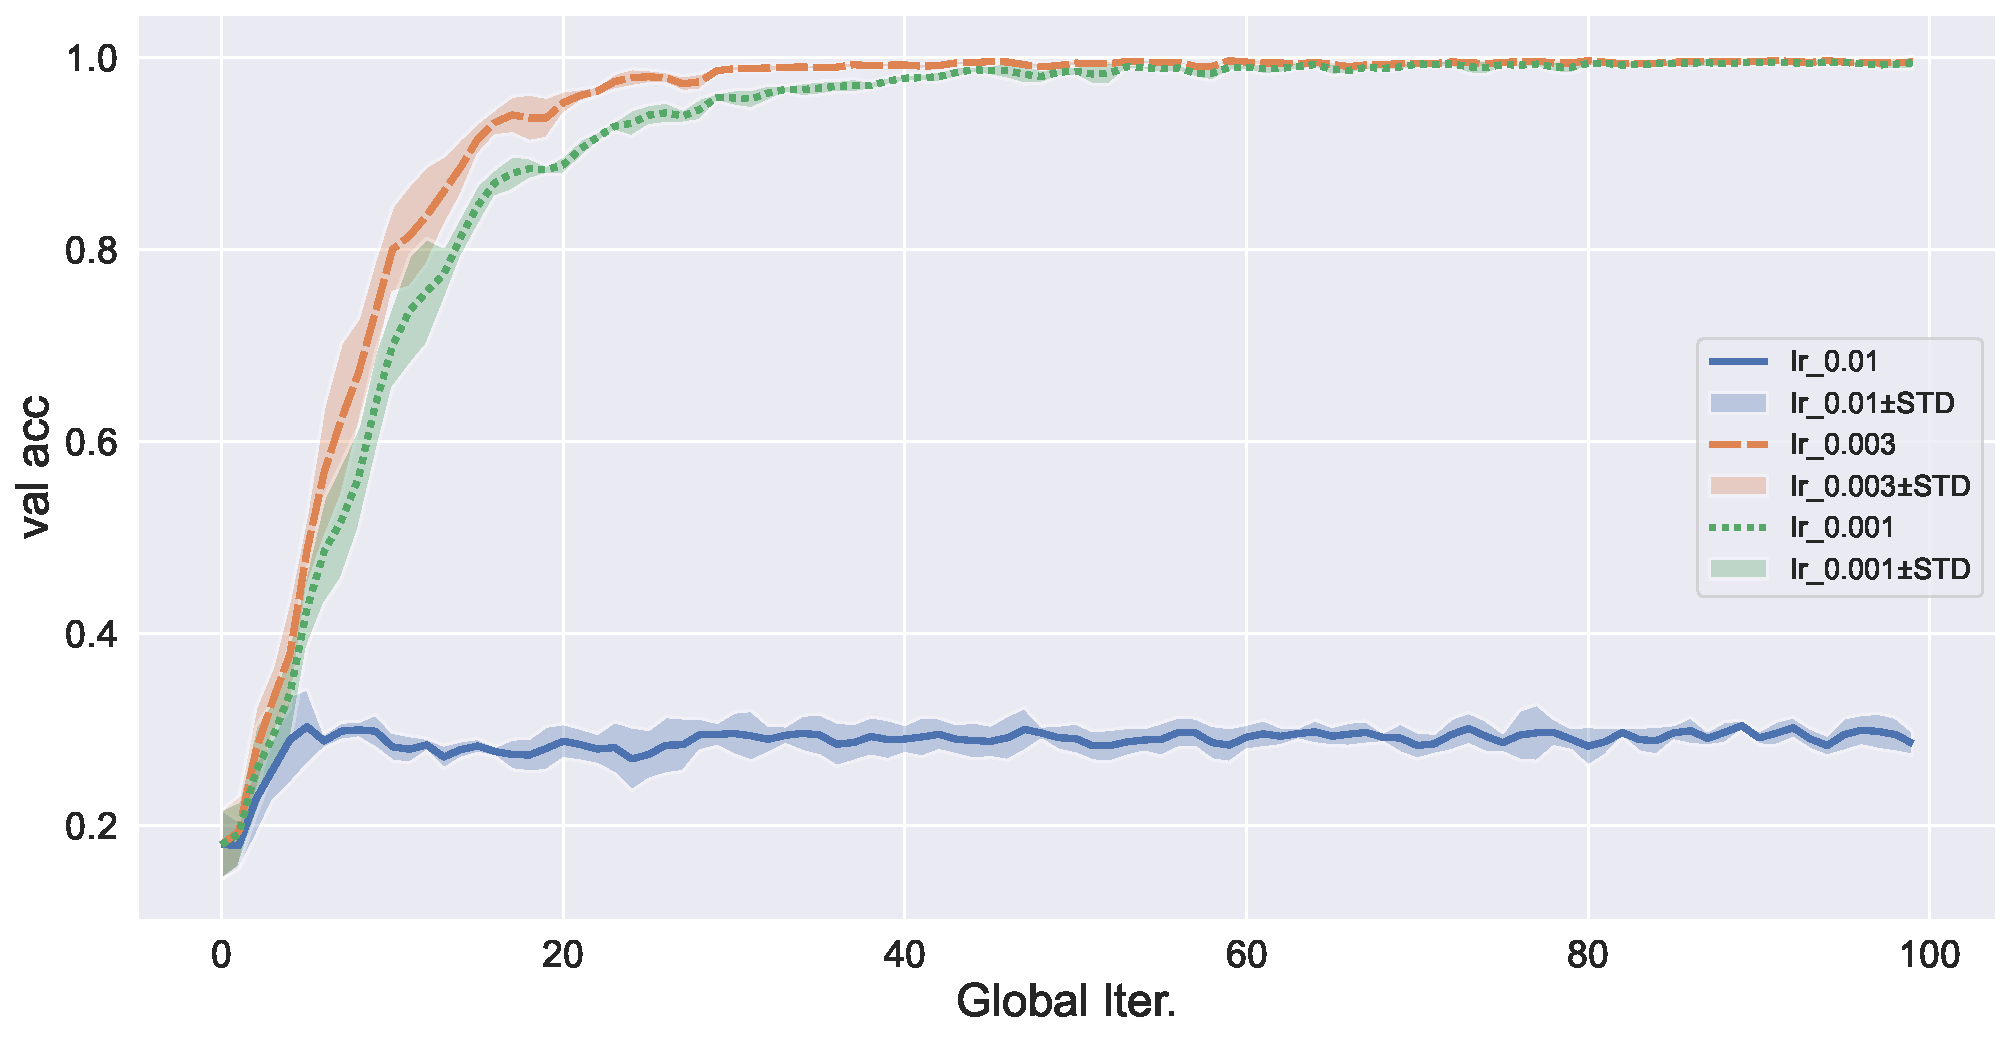
\includegraphics[width=.95\linewidth]{figures/adam-sample-30-compare-lr-val-acc.pdf}
  \caption{\texttt{FedAdam}算法在不同全局学习率下测试集上的准确率曲线}
  \label{fig:adam-sample-30-compare-lr-val-acc}
\end{subfigure}%
\begin{subfigure}{.5\textwidth}
  \centering
  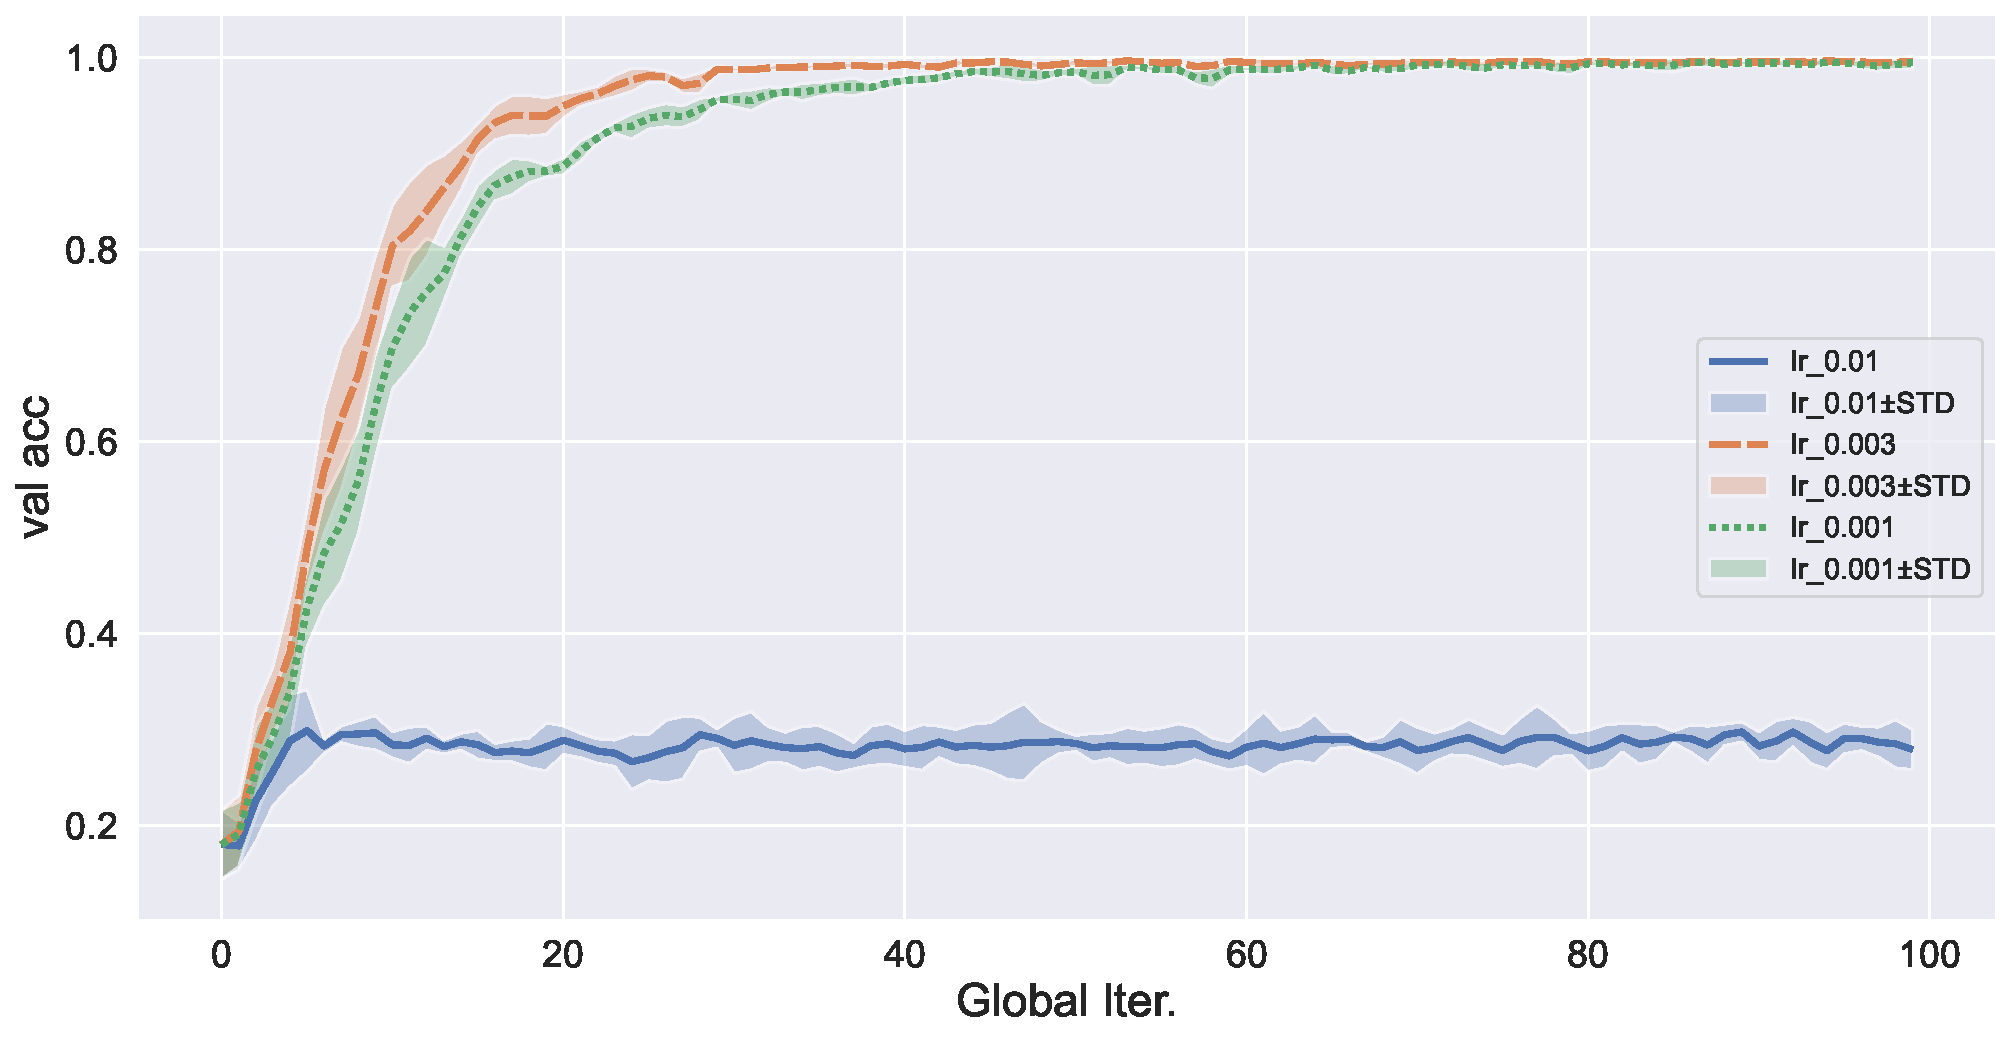
\includegraphics[width=.95\linewidth]{figures/yogi-sample-30-compare-lr-val-acc.pdf}
  \caption{\texttt{FedYogi}算法在不同全局学习率下测试集上的准确率曲线}
  \label{fig:yogi-sample-30-compare-lr-val-acc}
\end{subfigure}
\begin{subfigure}{.6\textwidth}
  \centering
  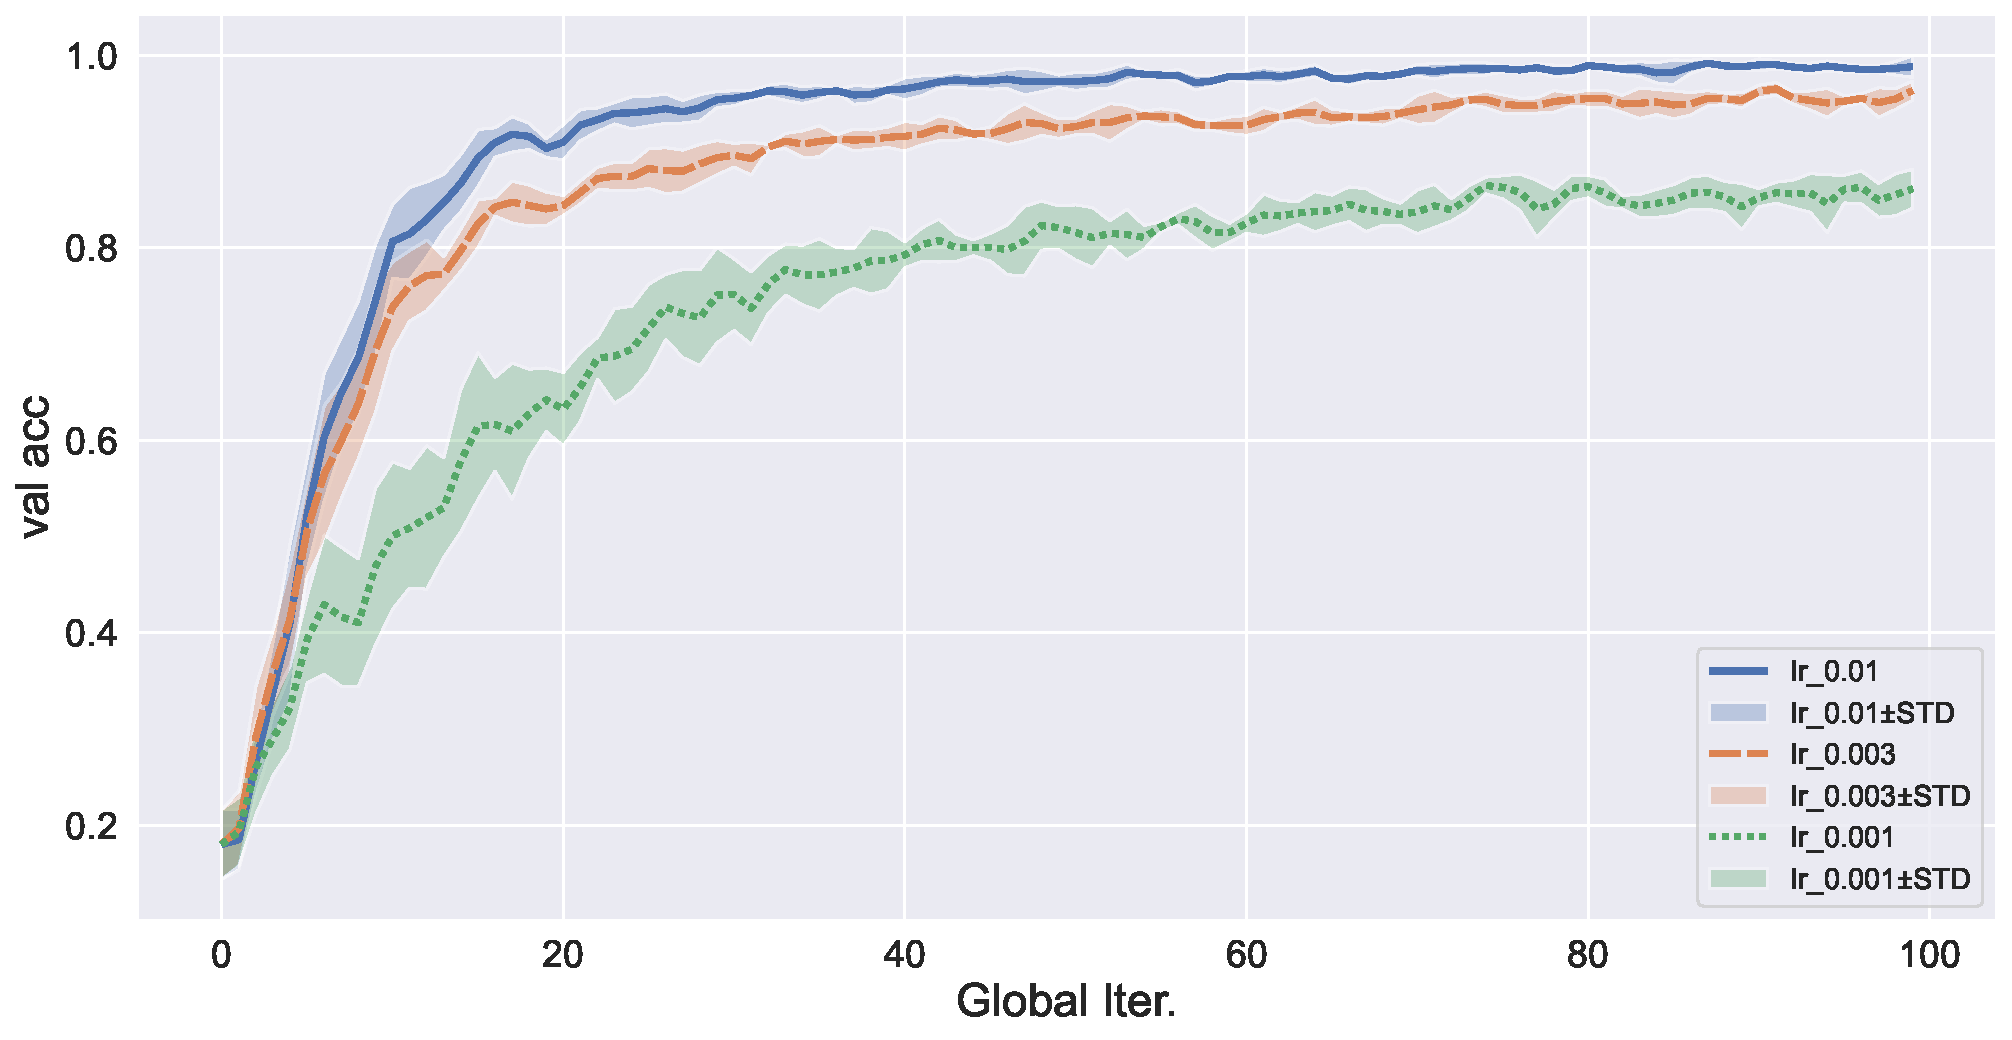
\includegraphics[width=.95\linewidth]{figures/adagrad-sample-30-compare-lr-val-acc.pdf}
  \caption{\texttt{FedAdagrad}算法在不同全局学习率下测试集上的准确率曲线}
  \label{fig:adagrad-sample-30-compare-lr-val-acc}
\end{subfigure}
\caption{几种联邦自适应类算法在不同全局学习率下测试集上的准确率曲线,子节点的训练参与率固定为$30\%$}
\label{fig:fedopt-sample-30-compare-lr-val-acc}
\end{figure}

可以看到,对于联邦自适应算法\texttt{FedAdam}与\texttt{FedYogi}来说,在$10^{-2}, 10^{-2.5}, 10^{-3}$这几个全局学习率中,最适合的是$10^{-2.5},$ 但是稍小的学习率$10^{-3}$只是稍微降低了算法的收敛速度,但并没降低算法的数值效果 (在测试集上的准确率)。联邦自适应算法\texttt{FedAdagrad}对于全局学习率这一超参数没有\texttt{FedAdam}与\texttt{FedYogi}这么敏感,但是其代价是,更小的学习率降低了算法的数值效果。

为了排除子节点的训练参与率对于这几种联邦自适应类算法对全局学习率敏感性的影响,对于子节点的训练参与率$10\%, 70\%, 100\%$我们都做了类似的数值实验,并且得到了相似的数值结果。唯一的例外是,当子节点的训练参与率被设置为$70\%,$ 并且随机数种子置为$0$时,\texttt{FedAdam}算法在全局学习率置为$10^{-2}$时得到了相同的 (相同指的是,试验在测试集上的最终准确率) 收敛的结果。相关的数值结果绘制在图\ref{fig:adam-sample-70-compare-lr-val-acc}~中。

\begin{figure}[ht]
    \centering
    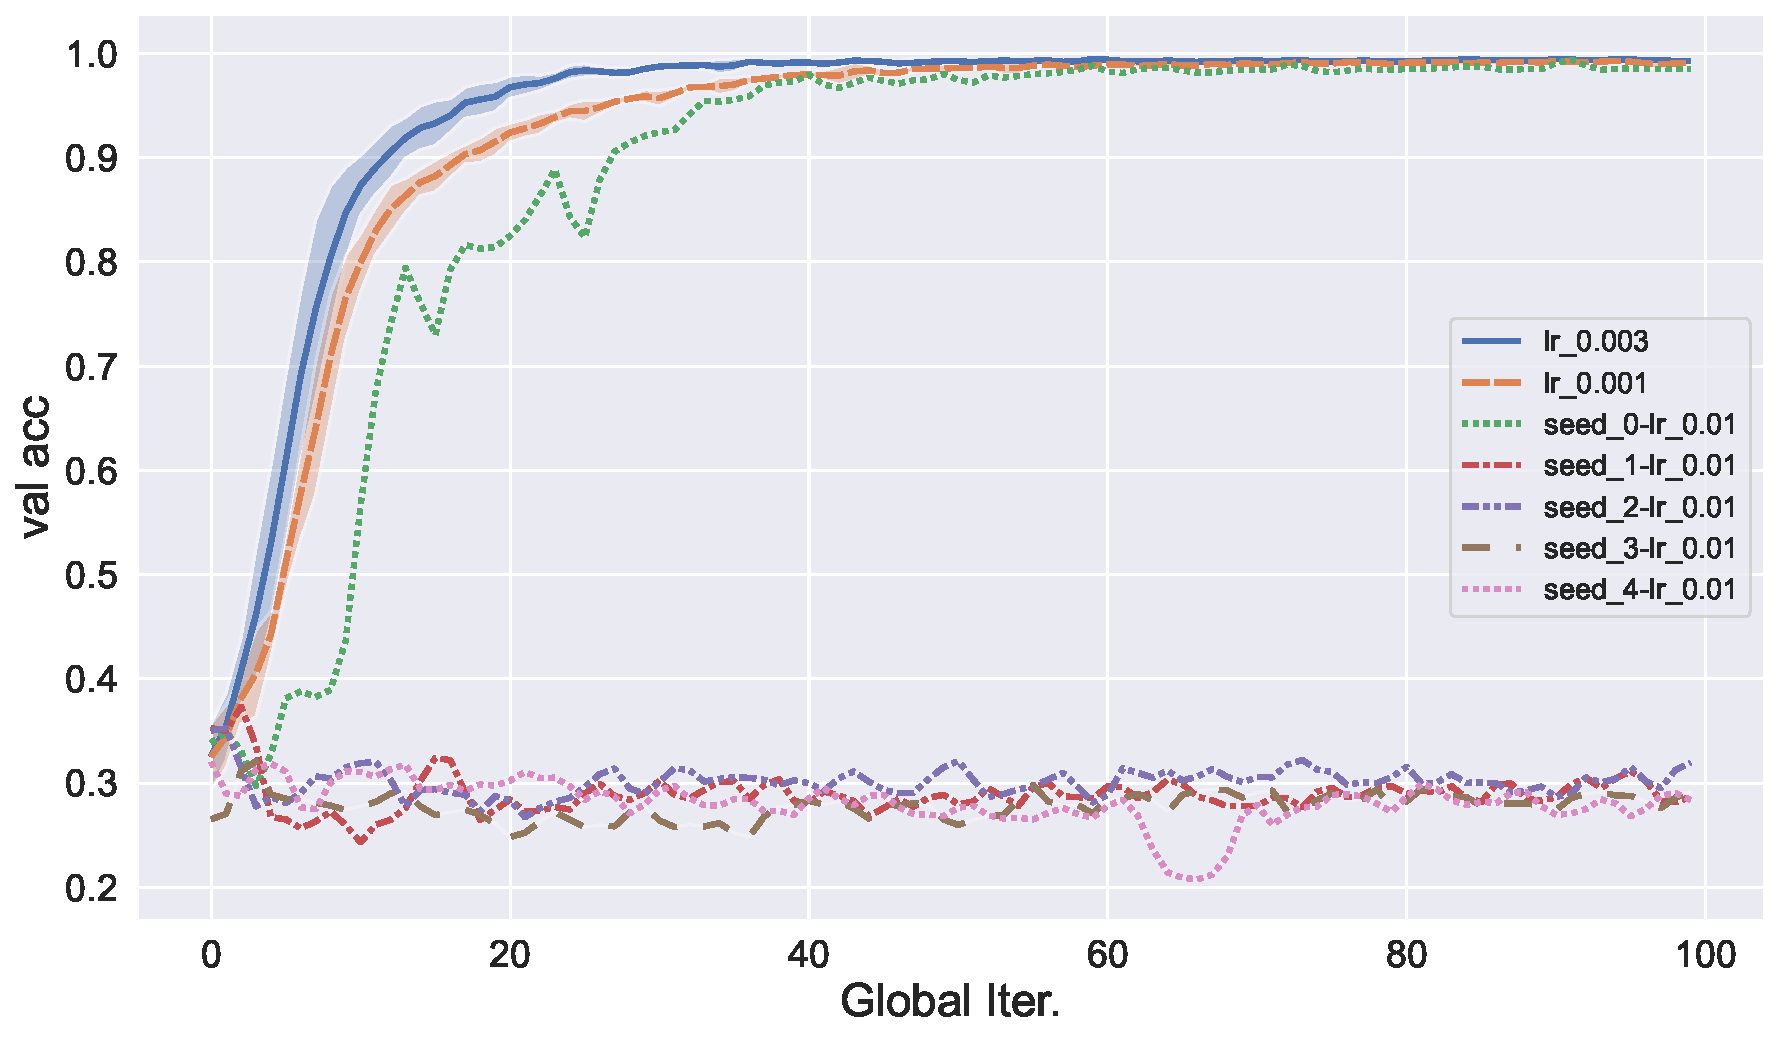
\includegraphics[width=0.7\textwidth]{figures/adam-sample-70-compare-lr-val-acc.pdf}
    \caption{\texttt{FedAdam}算法在不同全局学习率下测试集上的准确率曲线,子节点的训练参与率固定为$70\%$}
    \label{fig:adam-sample-70-compare-lr-val-acc}
\end{figure}
